\documentclass[tikz,border=3pt]{standalone}
\usepackage{amsmath,amssymb}
\usetikzlibrary{arrows.meta,calc}
\definecolor{curveblue}{HTML}{245C86}
\definecolor{accent}{HTML}{A65E2E}
\definecolor{curveteal}{HTML}{287B6D}
\definecolor{curveviolet}{HTML}{76578B}
\begin{document}
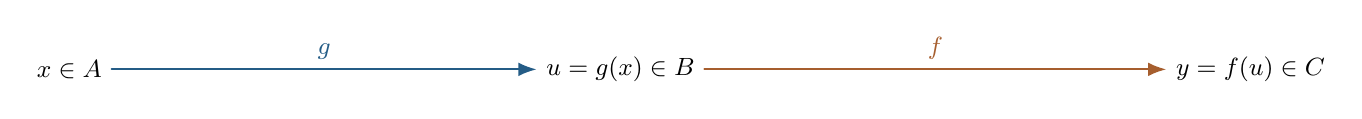
\begin{tikzpicture}[font=\small,>=Latex,line cap=round,line join=round]

\node (x) at (0,0) {$x\in A$};
\node (u) at (7,0) {$u=g(x)\in B$};
\node (y) at (15,0) {$y=f(u)\in C$};
\draw[->,curveblue,thick] (x)--node[above]{$g$}(u);
\draw[->,accent,thick] (u)--node[above]{$f$}(y);
\end{tikzpicture}
\end{document}
